\chapter{Theoretical Background}

\indent In 1932, Heisenberg formulated an idea that proton and neutron are in fact two states of the same particle, the nucleon. He proposed a new quantum number to label these states and he called it isospin ($I$) which in case of a nucleon carries a value of $\frac{1}{2}$. The Z components of the  isospins for a proton and neutron, labelled as $I_{3}$, are therefore $I_{3}=\frac{1}{2}$ and $I_{3}=-\frac{1}{2}$ respectively. Hence, the charge,$Q$, of the the nucleon can be written as:

\begin{equation}
\frac{Q}{e}=\frac{1}{2}+I_{3}
\end{equation}
where $e$ is the charge of an electron.

\indent In 1935, Yukawa, proposed that in order for the nucleons to be held together in a nucleus, some kind of "strong" force must exist and that the mediator particle for this force should be a spin-0 meson with a mass of $\sim150MeV$ \cite{dudek}. The existence of such particle has been proven 12 years later in 1947 when the charged pions were discovered by the collaboration of C. Powell, C. Lattes and G. Occhialini \cite{martin}.

\indent Pions are the lightest mesons with mass of $\sim135MeV$ and they act as mediators of the long-range part of the strong nuclear force. They are zero spin particles composed of two valence quarks and they can be found in three states; neutral, ($\pi^{0}$), and charged, ($\pi^{+}$ and $\pi^{-}$).

\indent Charged pions decay via weak interactions into muon and neutrino. The branching ratio of this decay mode is $\sim99.9\%$ with a mean lifetime of $2.6 \times 10^{-8}$s.
\begin{equation}
\pi^{+} \rightarrow \mu^{+} + \nu_{\mu}
\end{equation}
\begin{equation}
\pi^{-} \rightarrow \mu^{-} + \bar{\nu_{\mu}}
\end{equation}
Other possible decay modes are into an electron and anti-neutrino, and a positron and neutrino. However, the probability of these decay channels is very low $\sim0.001\%$.

\indent Neutral pions decay via electromagnetic interactions with a mean lifetime of $8.4 \times 10^{-17}$s. The dominant decay mode (branching ratio of $\sim99\%$) is into two photons:

\begin{equation}
\pi^{0} \rightarrow \gamma + \gamma
\end{equation}
The second most probable decay mode ($\sim1\%$) is into a photon and an electron-positron pair \cite{amsler}.

\section{Coherent pion photoproduction}

\indent Pion photoproduction occurs when a photon interacts with a nucleon and the reaction mechanism results in the emission of a pion in the final state. There are four possible channels of this reaction:

\begin{equation}
\gamma + p \rightarrow p + \pi^{0}
\end{equation}
\begin{equation}
\gamma + p \rightarrow n + \pi^{+}
\end{equation}
\begin{equation}
\gamma + n \rightarrow p + \pi^{-}
\end{equation}
\begin{equation}
\gamma + n \rightarrow n + \pi^{0}
\end{equation}

\indent Photoproduction can occur on a free nucleon (for example the proton nucleus of hydrogen) or for heavier elements from one of the nucleons bound within a nucleus. For heavier nuclei a coherent production process occurs only if the target nucleus is left in its ground state, $A_{gs}(\gamma,\pi^{0})A_{gs}$. If the initial and final states differ, the process is incoherent. Because of the charge conservation, reactions involving charged pions leave the target nucleus in a different state than the original, therefore; the only coherent production possible is the one featuring neutral pions \cite{claire}.

\indent The $\pi^{0}$ production process occurs with a close to equal probability on both protons and neutrons for the photon energy ranges analysed in this experiment. In the case of a coherent reaction there is not sufficient quantum information to identify which nucleon or shells of nucleons contributed to the reaction mechanism, therefore the amplitudes from all nucleons add coherently. The resulting production cross section, neglecting any final state interactions,  is then directly proportional to the square of mass number, A, and the square of the matter form factor. In this Plane Wave Impulse Approximation (PWIA) the cross section is expressed as \cite{drechsel2}:

\begin{equation}
\frac{d\sigma}{d\Omega}=A^{2} \frac{q}{k_{\gamma}} P^{2}_{3} |F_{m}(q)|^{2} sin^{2}(\theta_{\pi})
\end{equation}
where $q$ is the momentum transfered to the nucleus, $F_{m}(q)$ is the matter form factor of the nucleus, $P_{3}$ is the contributing pion photoproduction amplitude \cite{Proposal}. The matter form factor is a Fourier transform of the matter density distribution and because of that a diffraction pattern can be observed in the differential cross section.

\indent The use of photons to study neutron skin potentially allows for much more accurate measurements than strongly interacting probes. The strength of photon's electromagnetic interactions is very weak and as such they are not affected by the initial state interactions (ISI) and many-body interaction effects do not complicate the interpretation of the obtained data. Furthermore, the electromagnetic interactions are far better understood than strong interactions, and therefore, the results obtained with the use of electromagnetic probes are less susceptible to systematic effects in their theoretical interpretation \cite{claire}.

\indent Despite the photon probe in the entrance channel being close to ideal, the photoproduced pions are strongly interacting particles and therefore the effect of final state interactions (FSI) with the nucleus has to be accounted for. The real part of the pion-nucleus interaction is responsible for an angular shift in the ($\gamma,\pi^{0}$) angular distribution and the imaginary part, taking the absorption processes into account, explains the reduction in flux \cite{Proposal}. It has been shown previously that the strength of the FSI scales with pion energy and that the pion-nucleus scattering cross section is dominated by the $\Delta(1232)$ resonance corresponding to the pion energy of $\sim165MeV$. Photoproduced pions with energies away from the peak of the resonance have smaller interaction with the nucleus. 

\indent Although the FSI complicates the analysis of the matter distribution in the nucleus, they also provide a very effective way to study pion-nucleus interactions across the whole volume of the nucleus. All the available information about those interactions comes from charged pions scattering experiments but due to very short lifetimes pions with energies lower than $30MeV$ could not have been used in those measurements. However, the coherent $\pi^{0}$ production is not constrained with the limitations of charged pions scattering experiments. It offers an opportunity to investigate the pion-nucleus interactions for pion energies nearing $0MeV$ evaluated over the entire volume of the nucleus \cite{claire}.

\indent The study of the coherent $\pi^{0}$ photoproduction provides therefore a unique way to test not only nuclear matter distribution but pion-nucleus interactions as well. The main objective of the experiment presented in this report is however, to use the coherent $\pi^{0}$ photoproduction as a mean to study the nuclear matter distribution of tin isotopes in order to determine how the neutron skin thickness depends on the mass number. The current predictions of neutron skin thicknesses of tin isotopes are presented in Fig. \ref{tiniso} below.

\indent Across an isotopic chain from $A = 112$ to $A = 124$ we expect a change in the neutron skin of $\sim 0.05fm$ which should be easily detectable in the measurement.

\begin{figure}[H]
\begin{center}
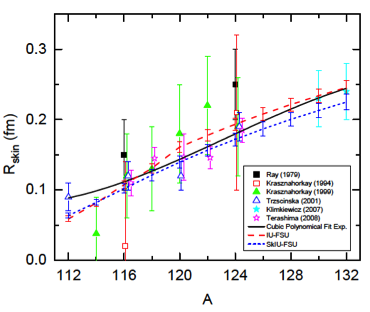
\includegraphics[scale=0.8]{pictures/png/tiniso.png}
\caption{The predictions of the neutron skin thicknesses for tin isotopes from the IU-FSU and SkIU-FSU models after the optimization compared to those determined with other, different experimental methods \cite{fattoyev}.}
\label{tiniso}
\end{center}
\end{figure}

\subsection{Reaction kinematics}

\indent The schematics of the kinematics of a pion photoproduction reaction are shown in a figure below (Fig. \ref{photorea}). The interacting particles, photon ($\gamma$) and a nucleon (N) have initial four-momenta k and $p_{i}$ respectively. The four-momentum is a combination of particle's energy and its three-momentum: P=(p,E).

\begin{figure}[H]
\begin{center}
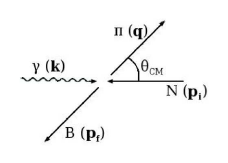
\includegraphics[scale=0.8]{pictures/png/photorea.png}
\caption{Simple diagram of a photoproduction reaction \cite{jo}.}
\label{photorea}
\end{center}
\end{figure}

\indent The Feynman diagrams shown below, illustrate that this reaction can proceed via three possible mechanisms (Fig. \ref{mandelstam}). First diagram, s-channel, describes a process where photon and nucleon combine into an intermediate particle (resonance) that eventually decays into two final state particles. In the case of t-channel, one of the interacting particles emits an intermediate particle which is subsequently absorbed by the other interacting particle. U-channel describes the same situation as t-channel with the exception of the final state particles being interchanged.

\begin{figure}[H]
\begin{center}
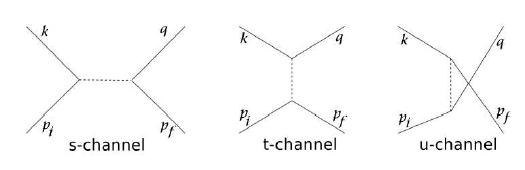
\includegraphics[scale=0.7]{pictures/png/mandelstam.png}
\caption{Feynman diagrams of the s-channel, t-channel and u-channel.}
\label{mandelstam}
\end{center}
\end{figure}

\indent The kinematics of any such production reaction can be easily described with the use of Lorentz-invariant Mandelstam variables s, t and u. The mechanisms are commonly referred to as: s-channel, t-channel and u-channel (Fig. \ref{mandelstam}). They are defined in terms of four-momenta as \cite{walker}:

\begin{equation}
s=(k+p_{i})^{2}=(q+p_{f})^{2}
\end{equation}
\begin{equation}
t=(p_{i}-p_{f})^{2}=(k-q)^{2}
\end{equation}
\begin{equation}
u=(p_{i}-p_{f})^{2}=(k-p_{f})^{2}
\end{equation}
where, $s$ is the square of the energy of the reaction, $t$ is the square of the momentum transfer, while the sum of the squares of the masses of particles is defined as a linear combination of those three variables.

\begin{equation}
s+t+u=\sum m^{2}_{i}
\end{equation}

\indent Only two of the Mandelstam variables are necessary to fully describe the reaction between photon and nucleon. In the relativistic approximation, $mc^{2}<<E$, these variables can be written as:

\begin{equation}
s=4p^{2}
\end{equation}
\begin{equation}
t=2p^{2}(1-cos\theta)
\end{equation}
\begin{equation}
u=2p^{2}(1+cos\theta)
\end{equation}
where $\theta$ is the pion scattering angle in the center of mass frame of reference. If $s$ is fixed, $t$ is a linear function of $cos\theta$, and therefore, the scattering functions can be represented completely in terms of $s$ and $cos\theta$ \cite{bertulani}.

\subsection{Reaction cross sections}

\indent For a pion, or any other meson, created in a photoproduction process, its angular distribution can be represented by a differential cross section:

\begin{equation}
\frac{d\sigma}{d\Omega}=|A(s,cos\theta)|^{2}
\end{equation}

\indent The probability of the transition from a given initial state $\left<i\right|$ to another final state $\left|f\right>$ can be represented by a scattering matrix $S$ in the Bjorken Drell notation \cite{bjorken}:

\begin{equation}
S_{fi}=\delta_{fi}-\frac{i}{(2\pi)^{2}} \delta^{4}(q-k+p_{f}-p_{i}) \sqrt{\frac{m_{N}^{2}}{4E_{\gamma}E_{\pi}E_{i}E_{f} } } <i|T|f>
\end{equation}
where, $T$ is the transmission matrix relating initial and final states, $m_{N}$ is the mass of a nucleon, and q, k, $p_{i}$, $p_{f}$ are four-momenta of the involved particles. The transmission matrix $T$ describes the amplitude of the photoproduction process, and can be written as:

\begin{equation}
T=\epsilon_{\mu}J_{\mu}
\end{equation}
where, $\epsilon_{\mu}$ is the photon polarization vector and $J_{\mu}$ is the electromagnetic current of a nucleon. Then the differential cross section can be defined as:

\begin{equation}
\frac{d\sigma}{d\Omega}=\frac{q}{k}\left(\frac{m_{N}}{4\pi W}\right)^{2}\sum |T|
\end{equation}
where, $W$ is the invariant mass of the system.

\indent The electromagnetic current of a nucleon, $J$, as proposed by Chew, Goldberg, Low, Nambu (CGLN), can be written in terms of nucleon spin matrices, $\sigma$, and meson unit vectors \^q and \^k \cite{chew}:

\begin{equation}
J=\frac{q}{k}\frac{4\pi W}{m_{n}}(i\sigma F_{1}+({\sigma} \cdot \hat{k})({\sigma} \times \hat{q})F_{2}+i \bar{k}(\bar{\sigma} \cdot \hat{q})F_{3}+i\bar{k}({\sigma} \cdot \hat{k})F_{4})
\end{equation}
where,
\begin{equation}
\bar{\sigma}=\sigma-(\sigma \cdot \hat{q})\hat{q}
\end{equation}
\begin{equation}
\bar{k}=\hat{k}-(\hat{k} \cdot \hat{q})\hat{q}
\end{equation}
and $F_{1}$, $F_{2}$, $F_{3}$, $F_{4}$, known as CGLN amplitudes, are the structure functions of energy and scattering angle, which can be written in terms of electric and magnetic multipoles and angular momentum through a partial wave expansion as:

\begin{equation}
F_{1}(\theta)=\sum\limits_{l=0}^{\infty} (lM_{l+}+E_{l+})P'_{l-1}(cos\theta)+((l+1)M_{l-}-E_{l-})P'_{l-1}(cos\theta)
\end{equation}
\begin{equation}
F_{2}(\theta)=\sum\limits_{l=0}^{\infty} ((l+1)M_{l+}+lM_{l-})P'_{l}(cos\theta)
\end{equation}
\begin{equation}
F_{3}(\theta)=\sum\limits_{l=0}^{\infty} (E_{l+}-M_{l+})P"_{l+1}(cos\theta)+(E_{l-}+M_{l-})P"_{l-1}(cos\theta)
\end{equation}
\begin{equation}
F_{4}(\theta)=\sum\limits_{l=0}^{\infty} (M_{l+}-E_{l+}-M_{l}-E_{l-})P"_{l}(cos\theta)
\end{equation}
where, $P'_{l}$ and $P"_{l}$ are derivatives of a Legendre polynomials, $l$ is the relative orbital momentum of a meson, $E_{\pm}$ and $M_{\pm}$ are electric and magnetic transitions respectively, and the + or - determines whether the spin of the baryon should be added or subtracted.

\indent The total angular momentum of a nucleon is $\frac{1}{2}$, and the total angular momentum of an incident photon is $L_{\gamma}$. In order to satisfy the selection rule, the resulting spin of a resonant state has to obey the following relation \cite{krusche}:

\begin{equation}
\left|L_{\gamma}-\frac{1}{2}\right|<J_{N*}<\left|L_{\gamma}+\frac{1}{2}\right|
\end{equation}
and the parity is given as:

\begin{equation}
\pi_{N*}=\pi_{N}\pi_{\gamma}
\end{equation}
where, $\pi_{N}$, parity of a nucleon, is equal to 1, and $\pi_{\gamma}$, the parity of the photon is equal to:

\begin{equation}
\pi_{\gamma}=(-1)^{L_{\gamma}}
\end{equation}
\begin{equation}
\pi_{\gamma}=(-1)^{L_{\gamma}+1}
\end{equation}
respectively for an electric and magnetic multipoles.

\indent The selection rules for the angular momentum and parity of the resonant state with respect to the outgoing meson are given as:

\begin{equation}
\left|L_{\pi}-\frac{1}{2}\right|<J_{N*}<\left|L_{\pi}+\frac{1}{2}\right|
\end{equation}
\begin{equation}
\pi_{N*}=\pi_{N}\pi_{\pi}(-1)^{L_{\pi}}=(-1)^{L_{\pi}+1}
\end{equation}
where $\pi_{\pi}$ is -1.

\indent Combining the above equations sets a limit on the spin and parity of the resonance:

\begin{equation}
\left|L_{\gamma}\pm\frac{1}{2}\right|<J_{N*}<\left|L_{\gamma}\pm\frac{1}{2}\right|
\end{equation}
\begin{equation}
\pi_{N*}=\pi_{N\gamma}=(-1)^{L_{\pi}+1}
\end{equation}

\indent When a cross section is dominated by a single resonance, its quantum numbers are reflected in the angular distribution because of the dependence of the Legendre polynomials in the CGLN amplitudes. It means that the electric ($L={L_{\pi}\pm1}$) and the magnetic ($L={L_{\pi}}$) multipoles, and the spin and parity are related to the angular distribution of mesons. Most photoproduction mechanism, however, have more than one multipole contributing to the resonance and in order to distinguish between the different contributions, several channels must be investigated.

\indent Isospin, not conserved in the electromagnetic interactions, is conserved however, in the hadronic interactions. The isospin of the initial state, determined from the isospin of the nucleon, is $I_{i}=\frac{1}{2}$ while the contributions from the pion and nucleon's isospins determine the value of the isospin of the final state, $I_{f}$, which can therefore take values of $\frac{1}{2}$ or $-\frac{1}{2}$. The value is determined by the photon which behaves as a linear combination of an isoscalar ($I_{s}$), which conserves the isospin, and an isovector ($I_{v}$), which can change the isospin by one, components. The whole system can be then described by the three isospin amplitudes \cite{nagl}:

\begin{equation}
A^{0}=<\frac{1}{2},I_{3}|I_{s}|\frac{1}{2},I_{3}>
\end{equation}
for the isoscalar electromagnetic current, and:
\begin{equation}
A^{1}=<\frac{1}{2},I_{3}|I_{v}|\frac{1}{2},I_{3}>
\end{equation}
\begin{equation}
A^{3}=<\frac{3}{2},I_{3}|I_{v}|\frac{1}{2},I_{3}>
\end{equation}
for the isovector electromagnetic current.

\indent As defined in \cite{davidson}, if the amplitudes are written as:

\begin{equation}
A^{+}=\frac{A^{1}+2A^{3}}{3}
\end{equation}
\begin{equation}
A^{-}=\frac{A^{1}-A^{3}}{3}
\end{equation}
the physical amplitudes for pion photoproduction can be expressed as:

\begin{equation}
A(p\gamma \rightarrow n\pi^{0})=<p\pi^{0}|I|p\gamma>=(A^{0}+A^{+})
\end{equation}
\begin{equation}
A(n\gamma \rightarrow n\pi^{0})=<n\pi^{0}|I|n\gamma>=(A^{+}+A^{0})
\end{equation}
\begin{equation}
A(p\gamma \rightarrow n\pi^{+})=<n\pi^{+}|I|p\gamma>=\sqrt{2}(A^{0}+A^{-})
\end{equation}
\begin{equation}
A(n\gamma \rightarrow p\pi^{-})=<p\pi^{-}|I|n\gamma>=\sqrt{2}(A^{0}-A^{-})
\end{equation}
The above set of equations allows for the separation of the amplitudes for individual photoproduction reactions provided that the measurements on both proton and neutron targets are carried out.

\subsection{Partial Wave Analyses}

\indent In order to extract information on the masses, widths and amplitudes from the experimental data, different reaction models have been developed and used. The most common approach involves separation of background and resonant terms of a transition matrix.

\indent Considering a reaction of the form $A\rightarrow B\rightarrow C$, where $A$ is the initial state of the nucleon-photon system,$B$ is the intermediate resonant state and $C$ is the final state of the nucleon-meson system, the photoproduction process can be described with a below Hamiltonian:

\begin{equation}
H=H_{0}+V_{bg}+V_{R}(E)
\end{equation}
where, $H_{0}$ is a free Hamiltonian expressing the total kinetic energy of the interacting particles, $V_{bg}$ is the potential due to the background created by the non-resonant contributions to the reaction, and $V_{R}$ is potential due to the resonant term.

\indent The transition matrix for the process is given by:

\begin{equation}
T_{AC}=V_{AC}+\sum\limits_{B}V_{AC}g_{B}(E)T_{BC}(E)
\end{equation}
where, $g_{B}$ is the propagator of the channel B of the reaction, and $\sum\limits_{B}$ sums all the possible channels of the reaction $A\rightarrow C$ via $B$. Alternatively, the transition matrix can be split into the background and resonant terms what allows the calculations for the background and resonant contributions to be carried out independently.

\begin{equation}
T^{AC}=t_{bg}^{AC}+t_{R}^{AC}(E)
\end{equation}

\indent Partial wave analyses (PWA) are methods that allow to decompose the background and resonant terms of the transmission matrix into a number of partial waves of defined multipoles and momentum. Generally, the resonant terms are modelled with a Breit-Wigner form while the background is described with Born terms and vector-meson contributions. The extraction of the parameters from the analysis is done in a two-stage procedure of fitting the experimental data. 
\indent The most commonly used for the pion photoproduction PWAs are MAID, developed at the University of Mainz \cite{maid}, and SAID written by the CNS Data Analysis Center at George Washington University \cite{said}.

\indent MAID is a unitary isobar model which describes the transmission matrix through a single $\pi N$ channel \cite {drechsel}:

\begin{equation}
T_{\gamma\pi}=V_{\gamma\pi}(E)+V_{\gamma\pi}(E)g_{0}T_{\pi N}(E)
\end{equation}
where, $V_{\gamma\pi}$ is the transition potential of the $\gamma N\rightarrow \pi N$ reaction, $T_{\pi N}$ and $g_{0}$ are the scattering matrix and the free propagator of the $\pi N$ interaction respectively.

\indent The scattering matrix and the transition potential can be broken down to its constituents: background and resonant terms, which can be expanded as partial waves. The resonances included in MAID, classified as 4* by the Particle Data Group (PDG) \cite{pda}, however, MAID can only fit the reconances up to $2GeV$.

\indent In the methods developed for SAID, there are no assumptions about resonances and channels included in the analysis framework. The transmission matrix, defined for the following three channels: $\gamma N$, $\pi N$ and $\pi \Delta$ (covering all open channels), can be written as \cite{arndt}:

\begin{equation}
T_{\gamma\pi}=A_{1}(1+iT_{\pi N})+A_{R}T_{\pi N,\pi N}
\end{equation}
where $A_{R}$ parametrizes the multipole amplitudes of the resonant terms, and $A_{1}$ parametrises background.

\begin{equation}
A_{R}=\frac{m_{\pi}}{q}\left[\frac{k}{q}\right]^{l}\sum\limits_{n=0}^{N}p_{n}\left[\frac{E_{\pi}}{m_{\pi}}\right]
\end{equation}
\begin{equation}
E_{\pi}=\frac{s-(m_{\pi}+M)^{2}}{2M}=E_{\gamma}-m_{\pi}\Big(1+\frac{m_{\pi}}{2M}\Big)
\end{equation}
where $E_{\pi}$ is the pion kinetic energy in the lab frame for the $\pi N\rightarrow \gamma N$, $s$ is the square of the center of mass energy, $M$ is the mass of the nucleon. $E_{\gamma}$ is the energy of the photon in the lab frame of reference for the $\gamma N \rightarrow \pi N$ reaction, and $p_{n}$ is a free parameter determined in the fit to the experimental data.

\begin{equation}
A_{1}=A_{B}+A_{Q}
\end{equation}
where, $A_{B}$ is a partial wave of a pseudoscalar Born amplitude, and $A_{Q}$ is a Legendre function.

\indent Detailed explanation of MAID and SAID can be found in \cite{maid,drechsel} and \cite{said, arndt}.

\section{Nuclear Matter Distribution}

\indent The charge distributions for many stable nuclei have been toroughly investigated in the electron and proton elestic scattering \cite{alkhazov, batty, igo}. And because of the very good understanding of the electromagnetic interactionsthe, the charge radii are measured with a high degree of accuracy \cite{devires, fricke}. The calculations of the matter radius from the proton scattering experiments, however, are much less accurate because the nucleon-nucleon interactions are not well understood.

\indent Since an accurate measurement of the nuclear matter distribution and the determination of the neutron skin have been shown to have further implication for the studies of structure of the neutron stars, and understanding the isospin dependent bulk and surface properties of nuclear matter \cite{iida} many experiments investigating it have been carried out \cite{neumaier, dobrovolsky, alkhazov2}.

\indent Those reasons alone would be a good motivation for a neutron skin measurement, however, using tin as the target offers additional research opportunities. Tin has many stable isotopes and its proton number is a magic number, making tin isotopes ideal for the studies of the systematic changes in neutron density distribution and the evolution of neutron skin along the isotopic chain. Furthermore, recent publications have shown that there exists a relation between the thickness of the neutron skin and the symmetry energy of the equation of state \cite{babrown, danielewicz, liewen2}.

\subsection{The nuclear Equation of State}

\indent From the definition, the equation of state (EOS) is a function of density ($\rho$) and isospin asymmetry ($\alpha$) and it is expressed as the energy (E) per nucleon in the infinite nuclear matter, $\frac{E}{A} (\rho,\alpha)$ where $\alpha$ is expressed as:

\begin{equation}
\alpha=\frac{N-Z}{A}
\end{equation}
where, $N$ is the number of neutrons, $Z$ is the number of protons and $A$ is the atomic mass number.

\indent The Bethe-Weizsaecker mass formula, more commonly known as semi-empirical mass formula (SEMF), based on the theory of the liquid drop model, have been first proposed in 1935 to explain the various properties of an atomic nucleus. According to the formula, the binding energy, $E_{B}$ can be approximated as:

\begin{equation}
E_{B}=a_{V}A^{3}-a_{s}A^{\frac{2}{3}}+a_{C}\frac{Z^{2}}{A^{\frac{1}{3}}}-a_{A}\frac{(A-2Z)^{2}}{A}-\delta(A,Z)
\end{equation}
where, $a_{V}$ is the volume coefficient (based on the strong force), $a_{S}$, also based on the strong force, is the surface term which provides a correction to the volume term, $a_{C}$ is the Coulomb or electrostatic term which introduces a correction due to electrostatic repulsion. $a_{A}$ is the asymmetry coefficient, which is based on the Pauli exclusion principle, and accounts for the imbalances between numbers of proton and neutrons in a nucleus. The pairing term $\delta(A,Z)$ covers the effects of spin-coupling \cite{bertulani}.

\indent This formula, being one of the first and most widely used equation of states, gives a good description of the symmetric nuclear matter at nuclear densities. However, for the matter at higher densities and in the case of the assymetric matter, SEMF doesn't describe the experimental data well. Therefore, research into adapting the equation of state to such assymetric and high density matter is one of the most important studies in the fields of nuclear and particle physics.

\indent An accurate measurements of the neutron skin could potentially put tighter constraints on the asymmetry term of the EOS and make it more aplicable in describing assymetric or high density matter encountered, for example, in the neutron stars.

\section{Nuclear Theories}

\indent Ever since the formulation of the quantum mechanics, much of the research in the fields of nuclear and particle physics have been focused on the studies of the structure of the atomic nuclei. In those early times, the conventional theories treated nucleus as a quantum mechanical many-body problem of Fermions interacting through a non relativistic two-body potential defined by the Schroedinger equation \cite{ring}. In reality, this approach is not applicably for any but the lightest nuclei because the many-body problem cannot be resolved analytically. However, other methods developed and used in recent years, such as variational Monte Carlo and Green's function Monte Carlo techniques, have been successfully employed in solving non-relativistic many-body problems for nuclei with mass number greater than $10amu$ \cite{carlson, pieper}. For heavier nuclei those methods no longer hold and different approaches are required.

\indent The Skyrme \cite{skyrme} or Gogny \cite{gogny} interactions start off from the density dependent energy functions for iterative calculations of the Hartree-Fock. The parameters of these functions are then fitted to the experimental nucleon-nucleon scattering data.

\indent The relativistic mean field (RMF) theory is a model of the nucleon-nucleon interactions assuming that nuclei are point-like particles described by Dirac spinors and all the interactions between them occur via mesonic fields. Even though there are many meson fields possible, most calculations only use the $\sigma(x)$, $\omega^{\mu}(x)$ and $\vec{\rho^{\mu}}(x)$ fields and the vector potential due to the photon exchange between the nucleons, $A^{\mu}(x)$ in order to simplify the calculations \cite{meucci}. Just like Skyrme and Gogny forces, RMF theory also uses the Hartree-Fock variational methods to resolve the nuclear wavefunctions.

\indent Most of the existing models used to describe the structure of nuclei are based either on the RMF theories or on the Skyrme or Gogny interactions. However, even though various models offer a fair degree of consistency when reproducing general properties of nuclear matter such as proton charge radius, they diverge when calculations of the neutron radius are considered \cite{pomorski, horovitz}. Fig. \ref{skinmass} shows discrepancies between neutron skin thickness calculations obtained from different models.

\begin{figure}[H]
\begin{center}
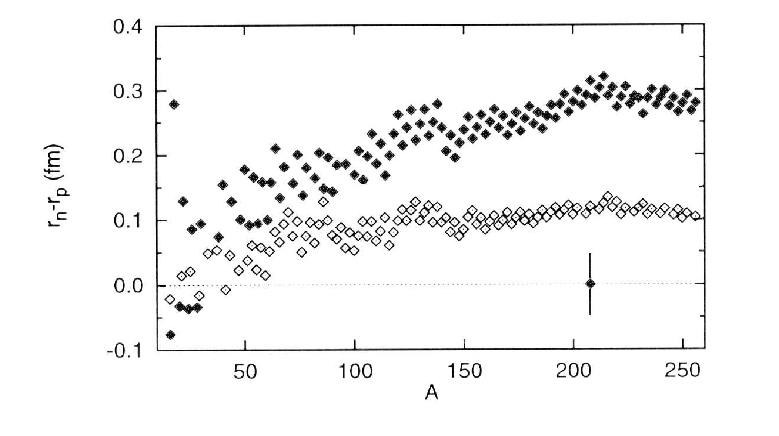
\includegraphics[scale=0.55]{pictures/png/skinmass.png}
\caption{The variation of neutronskin thickness as predicted by different models. Filled markers are for the RMF theory calculations and empty markers show the predictions of the Skyrme forces. Taken from the reference \cite{horovitz}.}
\label{skinmass}
\end{center}
\end{figure}

\section{Kamalov's DREN Calculations}

\indent The theoretical calculations done for this analysis were made using the code provided by S.Kamalov.
\indent The DREN (Delta Resonance Energy Model) calculations use the matter form factor (Fourier transform of the matter density distribution) as an input. The calculations are done under the assumption that both, matter and charge density distributions, $\rho(r)$, can be parametrised as a symmetries Fermi function:

\begin{equation}
\rho(r)=\rho_{0}\frac{sinsh\left(\frac{c}{b}\right)}{cosh\left(\frac{c}{b}\right)+cosh\left(\frac{r}{b}\right)}
\end{equation}
where, $b$ is the diffuseness parameter, $c$ is the half height radius and $\rho_{0}$ is defined as:

\begin{equation}
\rho_{0}=\frac{3}{4\pi c^{3}}\left(1+\frac{\pi b}{c}^{2}\right)^{-1}
\end{equation}
Then the root mean square radius, $r_{rms}$, of the distribution is expressed as:

\begin{equation}
r_{rms}=\frac{3c^{2}}{5}\left(1+\frac{7}{3}\left(\frac{\pi b}{c}\right)^{2}\right)
\end{equation}

\indent The matter and charge distributions used inthe calculations come from the recently provided by J. Piekarewicz RMF parameter set FSU-Gold \cite{piek2}. The parameter set FSU-Gold introduces an isoscalar-isovector coupling term, $\Lambda_{v}$, which simulates the density dependence of the symmetry energy \cite{sheng}. This parameter set has already been used and tested in the studies of the neutron skin of heavy nuclei \cite{piek3}, the equation of state for tin isotopes \cite{piek4} and the investigation into different models of nuclear structure \cite{piek5}.

\indent The calculations have been made for discreet values of photn energy in the $E_{\gamma}$ range of $180-240 MeV$ in $2 MeV$ steps. The results of those calculations for different targets are shown in the figure below:

\begin{figure}[H]
\begin{center}
%\includegraphics[scale=0.55]{pictures/pdf/.pdf}
\caption{The kamalov's DREN calculations of the cross sections for different targets, different $E_{\gamma}$ and different FSU-Gold parameters sets.}
\label{kamalov_tg}
\end{center}
\end{figure}


\section{Previous Measurements}

\indent Neutron skin measurements have been performed with strongly interacting probes before. The obtained data were strongly affected by many-body strong interaction effects that made the analysis and interpretation of the results ambiguous and difficult to draw binding conclusions from. The experiment involving proton scattering data fitted with different neutron skin thicknesses concluded with data being unable to determine the size or even the existence of the neutron skin \cite{piek}.

\indent The measurement of parity violation in electron scattering provides an independent probe of neutron densities because the weak charge of the neutron is much larger than that of proton. The interpretation of such results is model-independent and unaffected by the uncertainties of strong interactions. The polarized electrons have been used as a probe of neutron distribution in the $^{208}$Pb Radius Experiment (PREX). It made use of parity violation to accurately determine the neutron radius of the lead nucleus. The first measurement of the parity-violating asymmetry, $A_{PV}$ in the elastic scattering of polarized electrons from $^{208}$Pb reports the thickness of neutron skin of $\Delta R = 0.33_{-0.18}^{+0.16}$fm, and therefore provides the first electroweak observation of the neutron skin. \cite{prex}.

\indent The experiment investigating nuclear periphery at Low Energy Antiproton Ring (LEAR) at CERN allowed for an estimate of the relation between the symmetry parameter and neutron skin. 26 isotopes with mass numbers in a range of 40-238 have been studied. Antiprotons were chosen as a probe for the experiment since the antiproton-nucleus interactions are very strong and even a small overlap between their wave functions leads to the annihilation of the antiproton with one of the peripheral nucleons resulting in a final state nucleus with either proton or neutron number lower by one unit compared to the initial state. If both products are radioactive nuclear spectroscopy can be employed to determine their relative yields which are directly related to the proton and neutron densities at the annihilation site. The experimental results are presented in (Fig. \ref{antiproton}); analysis of the data indicated that neutrons are distributed in a form of a halo rather than a skin \cite{trzcina}. However, as the antiprotons are absorbed only in the surface of the nucleus the systematics in such measurements are somewhat controversial.

\begin{figure}[H]
\begin{center}
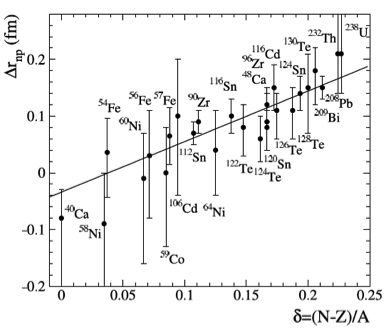
\includegraphics[scale=0.7]{pictures/png/antiproton.png}
\caption{Difference between the r.m.s. radii of the neutron and proton distributions ($\Delta r_{np}$) against the symmetry parameter $\delta$. Picture taken from the reference \cite{trzcina}.}
\label{antiproton}
\end{center}
\end{figure}



%now here you can refer to the first section like, see section \ref{sec1}......

